\section{Hardware}


The hardware components of the system were selected to facilitate ease of use low cost and mobility. Each camera node is comprised of a Raspberry Pi 4B microcontroller and a Pi Cam. Each camera node's purpose is to collect video and run the computer vision algorithm fast enough to produce and send real-time data. Another machine on the same network is used to host a central database where the statistics are stored, any retail laptop or computer is suitable for this purpose.

The Raspberry Pi 4B was selected for physical size, low cost, sufficiently computational power, networking capabilities and ease of integration with a camera module. The Raspberry Pi 4 also benefits from native operating system, support drivers for USB proprietary camera hardware and a large online community of makers. All of these factors made the Raspberry Pi 4 a easy choice for rapidly prototyping an IoT device. 

The Pi Camera was the selected image capture hardware primarily for it's compatibility with the Raspberry Pi environment, but it would not be viable without its low cost, 3-channel colour capture and frame rate. Figure \ref{fig:raspi_gear} shows the microcontroller with camera connected. Appendix \ref{appendices:hardware_specs} gives the full specifications of both of the Raspberry Pi 4 and Pi Cam.

\begin{figure}[H]
    \centering
    \centering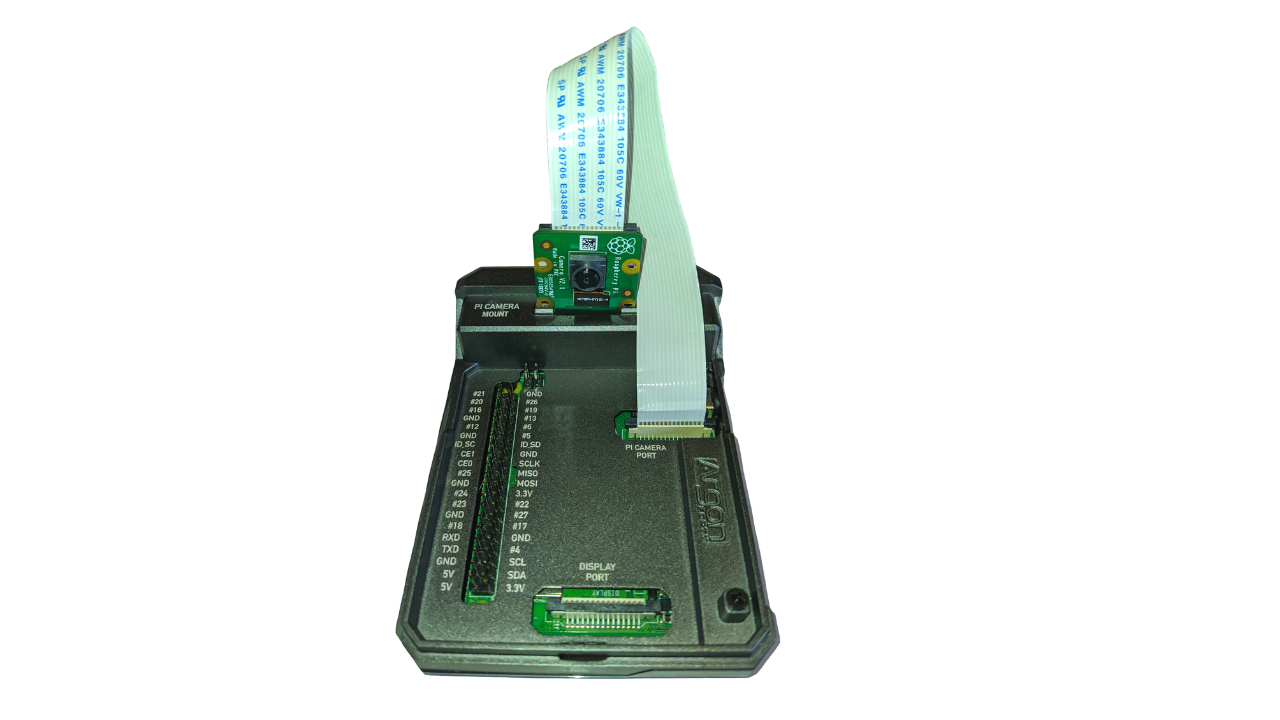
\includegraphics[width = 0.8\textwidth]{design/hardware/gear_improved}
    \caption{Raspberry Pi 4 and Pi Cam connected.}
    \label{fig:raspi_gear}
  \end{figure}
  